\chapter{Introduction}

\section{Background}

\subsection{High Performance Computing}

% HPCとはなにか
Recent advancement in science has significantly benefited from High Performance
Computing~(HPC). Scientists are able to simulate nature on HPC systems. HPC
helps scientists to develop a better understanding of nature and answer
fundamental questions about our surrounding environment by executing
high-resolution computational models of natural phenomena.

% HPCの応用分野
A wide spectrum of science has taken advantage of the massive computing
capability provided by HPC\@. Various phenomena ranging from atomic scale to
cosmological scale intractable to experimentally observe or reproduce are
simulated on HPC systems. For instance, molecular dynamics simulation reveals
the molecular-level structure and property of matter and their interaction.
This knowledge is used to design better drugs and materials. Earthquake and
Tsunami simulation allows us to predict the impact of seismic activities and
prepare for natural disasters. In addition to simulation applications, data
analysis and machine learning applications are also starting to leverage HPC
systems.

% HPCシステムの計算性能の推移
Scientists are trying to tackle increasingly larger and more complex problems.
This continuous demand from domain scientists has kept pushing the performance
HPC systems forward. Figure~\ref{fig:top500-rmax} shows the development of
computing performance of HPC systems based on the data published by the
Top500~\autocite{top500} list. The Top500 list is a biannual list of 500 most
powerful HPC systems measured by the maximal LINPACK benchmark performance
achieved. The plot clearly indicates the exponential increase in performance
over the past 20 years. Researchers and engineers are striving to sustain this
exponential growth in performance and exascale~(Exa FLOPS) in the near future.
To achieve this daunting technological challenge, every aspect of the HPC
system including hardware, operating system, middleware and application need
to be greatly improved, optimized and even redesigned.

\begin{figure}
    \centering
    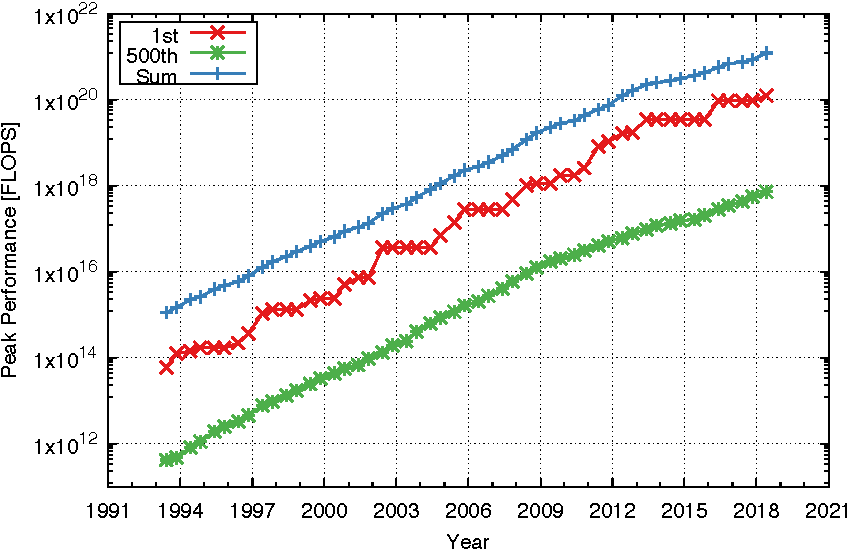
\includegraphics{top500_rmax}
    \caption{Performance Development of Top500 HPC Systems~\autocite{top500}}%
    \label{fig:top500-rmax}
\end{figure}

\subsection{Cluster Architecture}

% クラスタとはなにか
Modern HPC systems mostly adopt \emph{cluster} architecture to achieve their
massive computing performance. In fact, 87\% of the recent Top500 systems
(July 2018) are based on cluster architecture. A cluster is an aggregation of
interconnected computers working cooperatively. Computers that constitute a
cluster perform computation in parallel and exchange data with each other to
required for the computation.

% クラスタの構成要素
Figure~\ref{fig:cluster} shows the architectural overview of a typical
cluster. A cluster consists of multiple computers~(\emph{i.e.,\ computing
nodes}) and a high-performance network that integrates~(\emph{i.e.,\
interconnect}) them together as a single system. Since many users share a
single cluster, a \emph{job scheduler} is deployed to effectively manage the
computing resources in a cluster. A job scheduler accepts jobs from users and
determines when to run each job. The scheduler is also responsible for
allocating computing nodes to a job and launching jobs on allocated nodes.
Furthermore, a shared file systems is usually deployed to store the input and
output data of applications executed on the cluster.

\begin{figure}
    \centering
    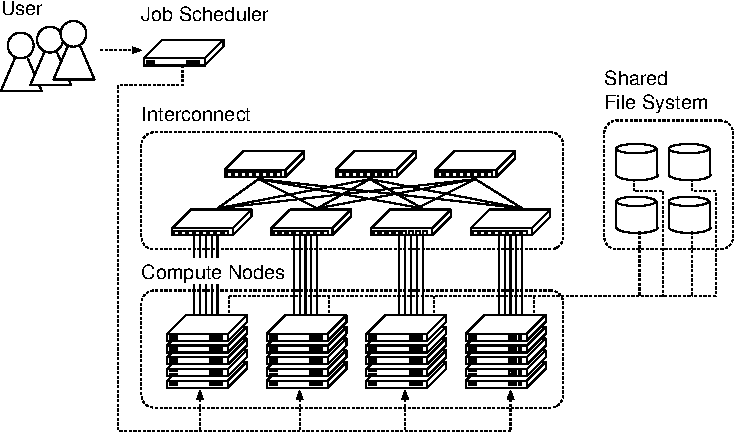
\includegraphics{cluster}
    \caption{Cluster Architecture}%
    \label{fig:cluster}
\end{figure}

% クラスタの規模拡大
There has been an increasing trend in the number of computing nodes that
compose a cluster. Although the computing performance of a single processor
and computing node have been steadily improving, the growth is not fast enough
to meet the high demand for computing power from the users. Therefore, the
designers of HPC systems need to increase the number of computing nodes to
further improve the total computing performance of the cluster. As a result, a
single cluster accommodates up to tens of thousands of computing nodes and
millions of cores nowadays.

% 相互結合網の重要性
The performance of communication between computing nodes over the interconnect
is essential to the scalability of the cluster. In general, computing nodes
need to frequently communicate with each other during the parallel computation
to exchange intermediate results. If the communication between computing nodes
becomes a bottleneck, simply adding more nodes to the cluster does not
increase the total performance of the cluster. Therefore, great effort has
been put to the research and development of high-performance interconnects.

\subsection{Message Passing Interface}\label{i-mpi}

Message Passing Interface (MPI)~\autocite{MPIForum2012} is a \emph{de
facto} standard specification for inter-process communication libraries
used to develop parallel distributed applications. MPI defines a suite
of communication primitives that helps programmers to develop
applications that require complex communications among computing nodes.

The communication primitives defined in MPI can be roughly categorized
into point-to-point communication and collective communication.
Point-to-point communication is a communication between one sender and
one receiver. On the other hand, collective communication involves a
group of multiple processes. Table~\ref{tbl:mpi-primitives} shows some
representative examples of MPI primitives.

\begin{table}
    \centering
    \caption{Examples of MPI primitives}%
    \label{tbl:mpi-primitives}
    \begin{tabular}{lll}
        \toprule
        Name & Category & Description \\ \midrule
        MPI\_Send/MPI\_Recv & Point-to-point & Blocking send/receive \\
        MPI\_Isend/MPI\_Irecv & Point-to-point & Non-blocking send/receive \\
        MPI\_Bcast & Collective & Broadcast \\
        MPI\_Reduce & Collective & Reduction \\
        MPI\_Allreduce & Collective & Broadcast result of reduction \\
        MPI\_Gather & Collective & \begin{tabular}[c]{@{}l@{}}Aggregate pieces of data from\\ processes into a single process\end{tabular} \\
        MPI\_Alltoall & Collective & \begin{tabular}[c]{@{}l@{}}Perform MPI\_Gather from all\\ processes\end{tabular} \\
        \midrule
    \end{tabular}
\end{table}

A remarkable feature of MPI is that it abstracts the underlying network
of high-performance computer clusters. This abstraction allows
programmers to develop applications without forcing them to study the
detailed architecture or structure of the underlying network. In MPI,
every process is identified by a \emph{rank} number, a non-negative
integer. The mapping between rank numbers and network addresses is
automatically handled by the MPI library. Communication can be
restricted into a certain group of processes, which is called a
\emph{communicator} in MPI\@. This abstraction makes MPI applications
portable and easy to port to different computer clusters.

Until today, countless scientific applications have been developed by
utilizing the communication primitives in MPI\@. The execution time of
these MPI primitives is an important performance factor because its
impact to the total application performance appears significantly
accompanied with the recent scale-out of computer clusters. In other
words, the total performance of MPI applications can be improved by
optimizing the performance of MPI communications. For this reason,
researchers have extensively investigated methods to improve the
communication performance of MPI from various aspects.

\subsection{Software-Defined Networking}

Software-Defined Networking (SDN) is a novel networking architecture
that separates the control plane and data plane into different devices.
In conventional networking architectures, the decision on how to handle
packets (control plane) and the packet transfer (data plane) are
implemented as unified and inseparable features. The separation of the
control plane and data plane has allowed SDN to deliver the following
three benefits:

\begin{itemize}
\item
  \emph{Programmable}: The control plane can be handled by a software
  controller. Network operators can program controllers tailored for
  their needs.
\item
  \emph{Dynamic}: SDN allows the controller to quickly reconfigure the
  network. For instance, it is possible to dynamically optimize traffic
  flow in the network based on the real-time traffic pattern.
\item
  \emph{Centralized}: A centralized controller configures the entire
  SDN-enabled network, thus reducing efforts to administer and manage
  the network. In conventional networking architectures, the operators
  need to configure each network device separately because the control
  plane is distributed on individual devices.
\end{itemize}

\begin{figure}
    \centering
    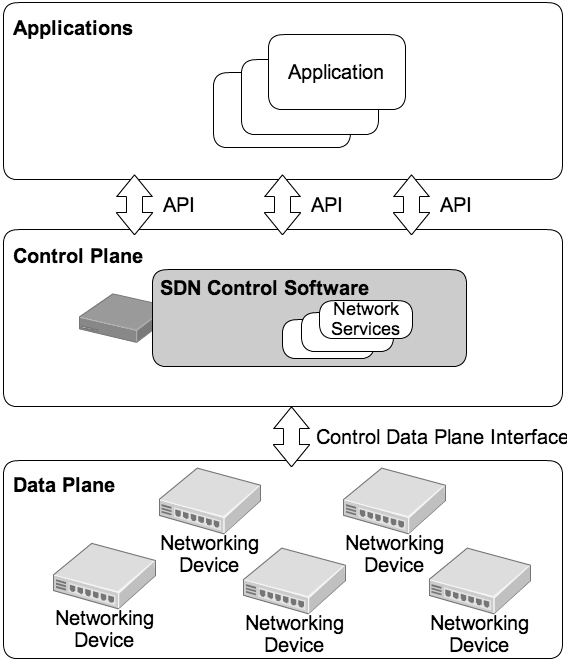
\includegraphics[width=.6\linewidth]{sdn-architecture.png}
    \caption{Software Defined Networking Architecture.}%
    \label{fig-sdn-architecture}
\end{figure}

\emph{OpenFlow}~\autocite{McKeown2008} is a widely accepted open
standard of SDN\@. In an OpenFlow-enabled network, the data plane is
handled by OpenFlow switches. Every OpenFlow switch holds a logical
construct called \emph{flow table}, which is a collection of \emph{flow
entries}. Each flow entry defines what kind of packet control should be
performed on what kind of packets (Fig.~\ref{tbl:flow-table}). Every
time a packet arrives at an OpenFlow switch, the switch looks up a
matching flow entry in its flow table using the header fields of the
packet. Once a matching flow entry is found, the action of the matched
flow entry is applied to the packet.

The OpenFlow controller is responsible for the control plane. It manages
the flow table of switches by adding, removing and modifying flow
entries. The controller and switches communicate with each other by
asynchronously exchanging messages defined in the OpenFlow protocol. One
of the frequently used messages is the \emph{packet-in} message, which
is sent out from a switch to the controller when no matching flow entry
is found for an incoming packet. In response, the controller can send a
\emph{modify flow entry} message to install a new flow entry on the
switch.

\begin{figure}
    \centering
    \begin{tabular}{lllll}
        \toprule
        \multicolumn{3}{c}{Header Fields}            &  Action                  \\ \midrule
        Dst MAC           & Src IP     & Dst IP      &                          \\ \midrule
                          & 192.0.2.12 & 192.0.2.34  & Output to port 1         \\
                          & 192.0.2.34 & 192.0.2.56  & Output to port 2         \\
        ff:ff:ff:ff:ff:ff &            &             & Output to port 1 and 2   \\
        72:42:c1:e4:75:8c &            &             & Drop                     \\
        \bottomrule
    \end{tabular}
    \caption{An example of a flow table}%
    \label{tbl:flow-table}
\end{figure}

\subsection{Related Work}

\section{Research Objective}

\section{Organization of the Dissertation}
